%!TEX root = ../../thesis.tex
\section{Filters}
\label{sec:webaudio-filter}

\begin{quote}
  ``It's quite ironic: We got rid of our analog equipment, replaced it with digital, then spent the next couple of decades trying to get the digital to sound like the analog we got rid of.'' -
  David Williams
\end{quote}

Audio filters allow for the manipulation of the frequency spectrum of a sound in order to create a certain effect on the sound or to sculpt a certain note so that it creates a different atmosphere in combination with other sounds. Each filter has several parameters that influence the effect on the source sound.

\begin{figure}[htb]
  \centerline{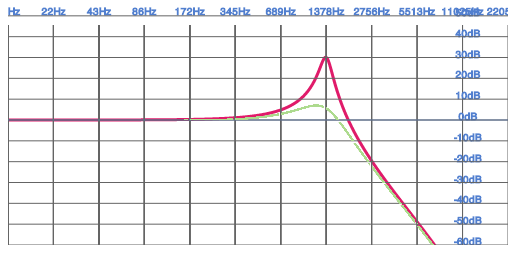
\includegraphics[width=0.9\linewidth]{images/filter-demonstration.png}}
  \caption[Visualization of a low-pass filter -
  \protect\newline{\small\url{http://webaudio-io2012.appspot.com/\#34} (01.03.2014)}
  \protect\newline{\small\emph{Chris Wilson}}]{Visualization of a low-pass filter (red: high Q, green: low Q)}
  \label{fig:filters-visualization}
\end{figure}

There is the \emph{cut-off} frequency parameter, which determines the level of frequency at which the filter should affect the sound. The example in \reffigure{fig:filters-visualization} shows a low-pass filter, which filters out lower frequencies. The cut-off frequency in this case is 1378Hz, the graph's peak, and the dB for higher frequencies is rapidly getting lower so they are not heard anymore. The next important parameter is the \emph{quality} factor of the filter which influences the steepness of the peak. The red line shows a filter with a higher \emph{quality} parameter than the green one. A low \emph{cut-off} frequency leads to a duller sound when a low-pass filter is applied. The \emph{quality} factor can influence the ``kick'' of the effect and stress the frequencies around the \emph{cut-off} point. Low-pass filters were the first filters that were added to synthesizers and because their cutoff was regulated with a knob the term \emph{opening} (lower value, more frequencies) and \emph{closing} (higher value, less frequencies) the filter was coined \cite[chapter: 2, Filter Types]{cannAnalogSynthesis}. The opposite of a low-pass filter is a high-pass filter, which filters out higher frequencies based on the above parameters.

Another class of filters are shelf filters. Both highshelf and lowshelf filters can be used to boost the volume for a range of frequencies. A highshelf filter, for example, amplifies frequencies that are higher than the frequency point which is set in a \emph{frequency} parameter (analogous to the \emph{cut-off} frequency above) by the amount of dB of the \emph{quality} parameter which results in more treble \cite[chapter: 6]{smus2013webaudio}. The lowshelf parameter does the same only for lower frequencies and therefore affects the amount of bass\footnote{\cite[chapter: 6]{smus2013webaudio}}.

In addition to the already mentioned filters, the Web Audio API also supports band-pass filters, peaking filters, notch filters and all-pass filters which are described in detail in \cite[The BiquadFilterNode Interface]{wilson2014webaudiospec}.

\begin{lstlisting}[language=JavaScript, caption=Applying a filter to a buffer, label=lst:webaudiofilter]
  var buffer = (...);
  var filter = context.createBiquadFilter();
  // 0 -> lowpass
  filter.type = 0;
  filter.frequency.value = 220;
  filter.Q.value = 15;
  // set up node graph
  buffer.connect(filter);
  filter.connect(context.destination);
\end{lstlisting}

Filters in the Web Audio API are nodes that are wired between the raw signal and the output so that they can manipulate the incoming signal before it reaches the speakers. In \reflisting{lst:webaudiofilter} a low-pass filter is created (line 2) and connected to the speakers (line 9). A buffer is used as an input signal (line 8) but the initialisation code is left out to make the example shorter and it has already been covered in \refchapter{sec:webaudio-buffer}. The parameters \code{frequency} and \code{Q} are set to values which make the output sound very dull and bass-heavy because only very low frequencies pass the filter and the relatively high \code{Q}-value of 15dB amplifies the frequencies around 220Hz.